\documentclass[11pt,a4paper]{article}
\usepackage[T1]{fontenc}
\usepackage[utf8]{inputenc}
\usepackage[french]{babel}
\usepackage{lmodern,geometry,amsmath,booktabs,tabularx,xcolor,graphicx,fancyhdr,hyperref,listings}
\geometry{margin=2.15cm}
\definecolor{bleu}{HTML}{173B57}
\hypersetup{colorlinks=true,urlcolor=bleu,linkcolor=bleu}
\pagestyle{fancy}\fancyhf{}\fancyhead[L]{TP1 -- Étude de la consommation d'un core}\fancyhead[R]{M2 ESTel}\fancyfoot[C]{\thepage}
\setlength{\headheight}{14pt}
\setlength{\parindent}{0pt}\setlength{\parskip}{6pt}
\renewcommand{\arraystretch}{1.2}
\lstset{basicstyle=\ttfamily\footnotesize,breaklines=true,frame=single,columns=fullflexible}
\begin{document}
\hypersetup{pageanchor=false}\begin{titlepage}
{\large Université Côte d'Azur\\EUR DS4H -- Master 2 ESTel\\SMUEL302 -- Architecture multicores}
\vspace{2.1cm}

{\Huge\color{bleu}\bfseries Étude de la consommation d'un core\par}
\vspace{0.5cm}
{\LARGE TP1 -- Opérateurs et traitement d'image sur FPGA\par}
\vspace{0.9cm}
{\Large Maxime Barbe\par}
\vspace{0.3cm}
26 octobre 2026

\vspace{1.2cm}
\begin{center}
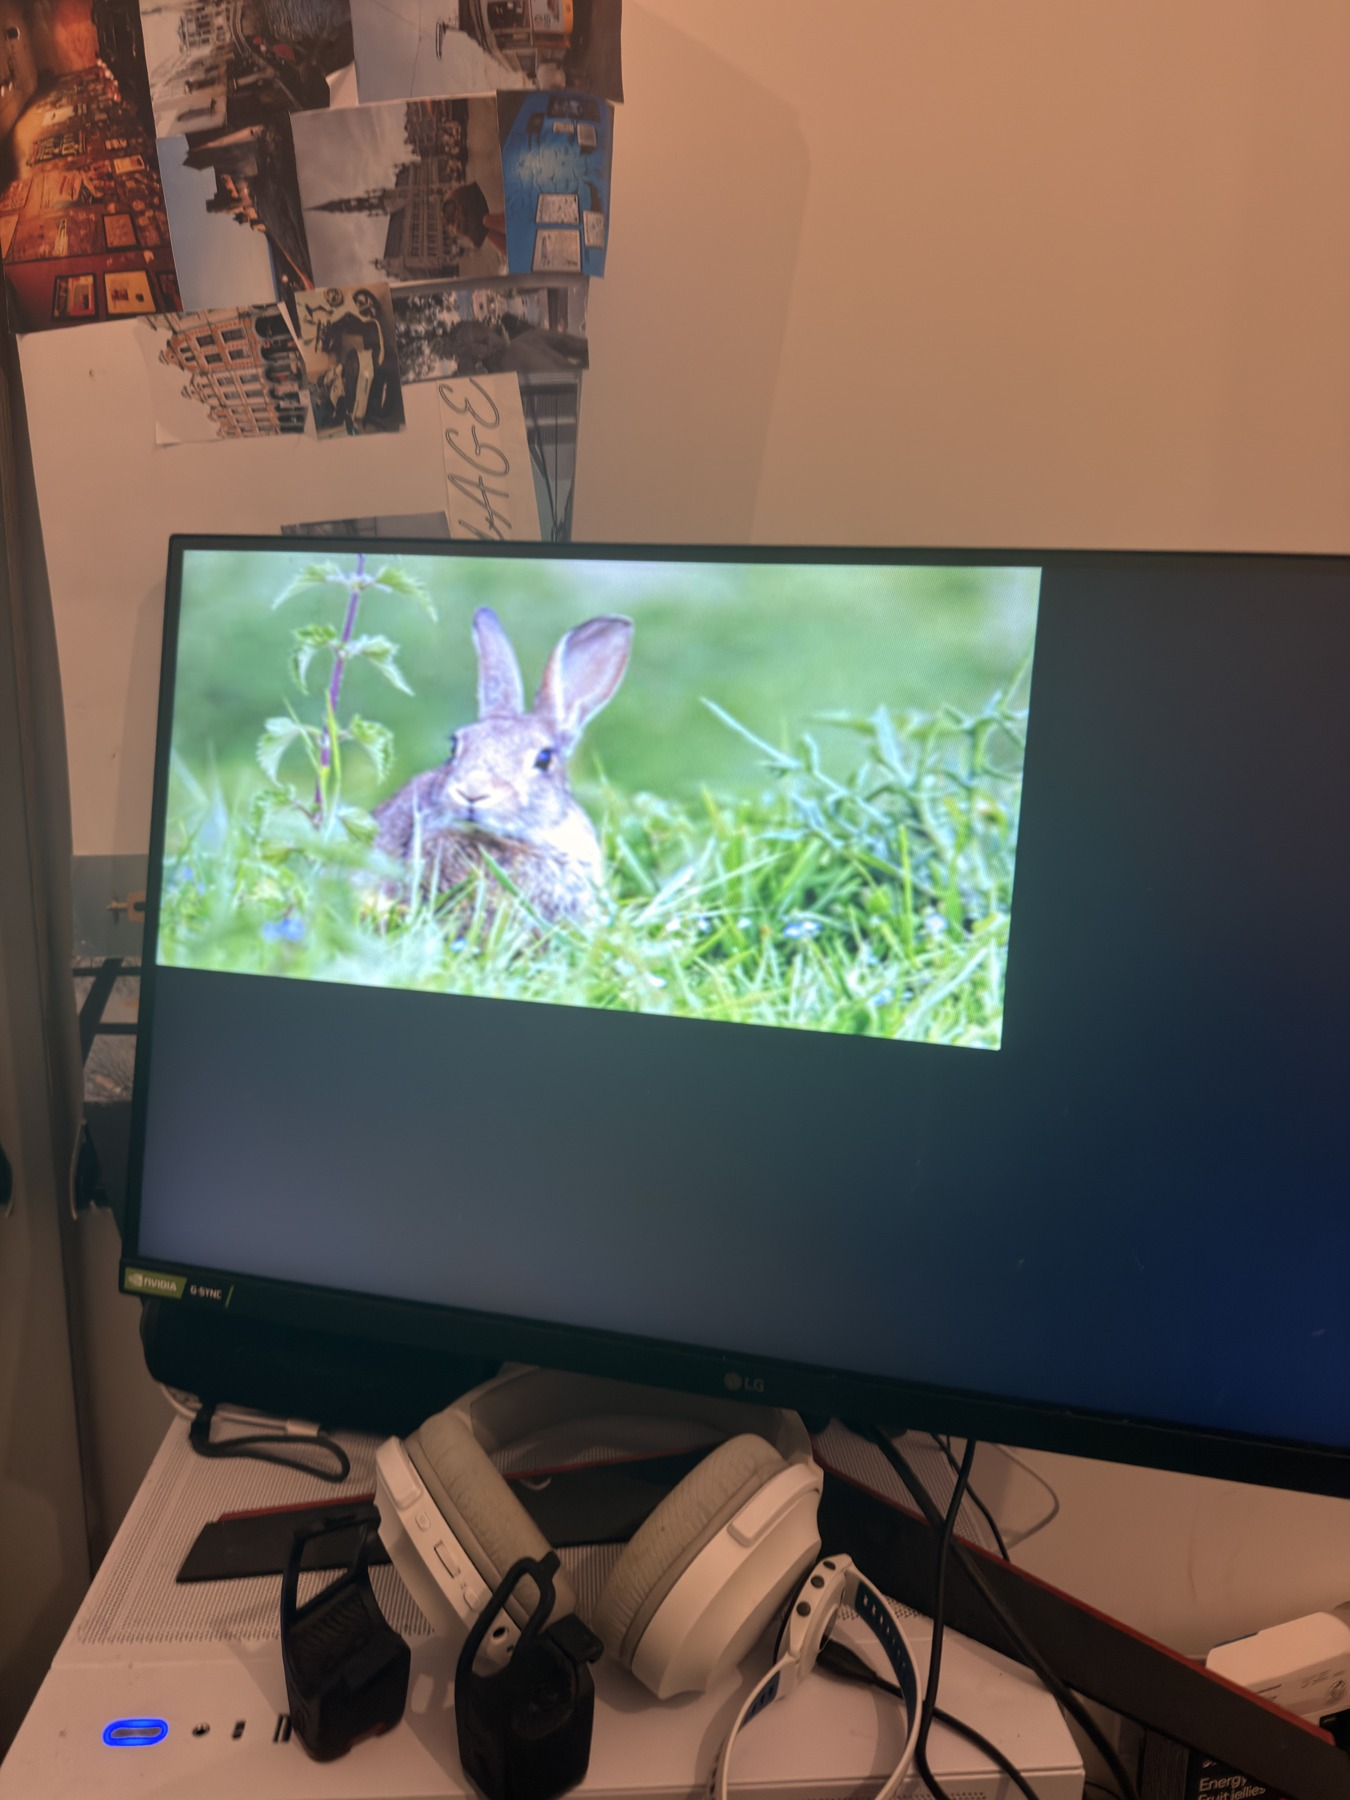
\includegraphics[width=0.70\linewidth,height=7cm,keepaspectratio]{images/affichage_on.jpg}
\end{center}
\vfill
\textbf{Plateforme :} Terasic DE10-Nano, Cyclone V 5CSEBA6U23I7.\\
\textbf{Outils :} Quartus Prime Lite 17.1, Power Analyzer, description VHDL/Verilog.

\small\textbf{État du compte rendu.} L'exercice 3 dispose d'un affichage observé et de quatre relevés d'alimentation. Les exercices 1 et 2 sont documentés à partir des sources disponibles ; leurs comparaisons de puissance et certains temps de réponse restent à compléter. Aucune valeur expérimentale n'est extrapolée pour combler ces manques.
\end{titlepage}\hypersetup{pageanchor=true}

\section{Objectif et méthode}
Le TP étudie la relation entre architecture, débit et consommation. L'exercice 1 compare des opérateurs 32 bits, le pipeline et le parallélisme. L'exercice 2 applique ces principes à un filtre vidéo. L'exercice 3 réalise une chaîne complète sur FPGA et mesure son alimentation [1].

\subsection{Puissance, énergie et périmètre}
Le cours distingue puissance statique et puissance dynamique [3, diapositives 8--9]. La première subsiste sans commutations utiles ; la seconde dépend notamment de l'activité, de la capacité commutée, de la tension et de la fréquence. L'énergie se calcule sur une durée :
\[
 P=P_{\mathrm{stat}}+P_{\mathrm{dyn}},\qquad
 E=\int_0^T P(t)\,dt \simeq \overline P\,T.
\]
Pour $N$ opérations valides terminées pendant la fenêtre $T$ :
\[
 E_{\mathrm{op}}=\frac{\overline P T}{N}
 =\frac{\overline P}{R_{\mathrm{op}}}.
\]
Pour une chaîne vidéo continue de débit $r$ images/s, $E_{\mathrm{image}}\simeq\overline P/r$. Cette normalisation est indispensable : une architecture plus puissante peut néanmoins consommer moins d'énergie par résultat si elle termine davantage de travail.

Le Power Analyzer estime une puissance du composant selon son modèle et l'activité fournie. Le testeur d'alimentation de l'exercice 3 inclut la carte et les pertes en aval de son point de mesure. Ces deux périmètres ne sont pas directement comparables.

\subsection{Données effectivement disponibles}
\begin{center}
\begin{tabularx}{\linewidth}{@{}l X@{}}
\toprule
Partie & Éléments exploitables\\
\midrule
Exercice 1 & Additionneur enregistré, testbench à 100 MHz, multiplieur LPM\_MULT et ancien rapport Power Analyzer du 29 septembre.\\
Exercice 2 & Filtre 3$\times$3 combinatoire à neuf entrées 8 bits ; intégration dans l'exercice 3.\\
Exercice 3 & Sources complètes, provenance de compilation, photos d'affichage, quatre relevés de tension/courant et CSV.\\
\bottomrule
\end{tabularx}
\end{center}
Les résultats de compilation repris ici proviennent des rapports conservés. Ils ne correspondent pas à une nouvelle campagne Quartus réalisée pour ce compte rendu.

\subsection{Conditions d'une comparaison équitable}
Il faut conserver le composant, les contraintes, les conditions électriques et thermiques, une distribution d'entrées comparable et une fenêtre d'activité documentée. Le nombre d'opérations réellement terminées doit être compté après remplissage du pipeline. Le support du TP rappelle l'importance des stimuli et de l'import d'un fichier d'activité VCD dans Power Analyzer [2, diapositives 5--11].

\newpage
\begingroup\small\section{Exercice 1 -- Opérateurs, pipeline et parallélisme}
\subsection{Additionneur 32 bits}
Le fichier \texttt{add32.v} réalise une addition non signée sur 32 bits avec sortie enregistrée :
\begin{lstlisting}[language=Verilog]
always @(posedge clk)
    R1 <= A + B;
\end{lstlisting}
Le résultat est ramené à 32 bits : la retenue finale est perdue. Ainsi, \texttt{FFFFFFFF + 1} produit zéro modulo $2^{32}$. Le testbench prévoit une période de 10 ns, soit 100 MHz, et quelques cas simples. Il s'agit de stimuli fonctionnels courts, insuffisants pour représenter seuls une activité arithmétique générale.

\subsection{Comparaisons demandées et interprétation}
Le pipeline raccourcit le chemin combinatoire entre registres mais ajoute des bascules et de l'activité d'horloge. À fréquence identique, il n'augmente pas nécessairement le débit si l'architecture accepte déjà un opérande par cycle. L'intérêt doit être évalué avec une fréquence plus élevée admissible et avec les coûts de remplissage.

Pour $q$ voies indépendantes, une fréquence $f$ et un intervalle d'initiation $II$, le débit théorique en régime établi est :
\[
 R_{\mathrm{op}}=\frac{qf}{II}.
\]
La latence de $L$ cycles vaut $L/f$ ; elle ne doit pas être confondue avec l'intervalle entre résultats. Le parallélisme augmente les ressources et l'activité ; son intérêt énergétique dépend de l'augmentation effective du débit et des échanges de données.

\begin{center}
\small
\begin{tabularx}{\linewidth}{@{}l X@{}}
\toprule
Comparaison demandée & État des données disponibles\\
\midrule
Addition entière, latence 1 & Source et testbench disponibles ; puissance non retrouvée.\\
Addition entière, pipeline 2 et 4 & Résultats de synthèse et d'activité non retrouvés.\\
Addition flottante & Variantes et rapports non retrouvés.\\
Voies parallèles & Comparaison chiffrée non disponible.\\
Multiplication DSP / éléments logiques & Un résultat DSP ancien retrouvé ; variante logique absente.\\
\bottomrule
\end{tabularx}
\end{center}

\subsection{Résultat ancien du multiplieur}
Le projet conservé utilise un \texttt{LPM\_MULT} signé, entrées 32 bits et produit 64 bits. Le schéma porte un paramètre de pipeline de 1 ; cependant, le rapport Fitter correspondant indique zéro registre final. Il faut donc vérifier la réalisation obtenue avant d'affirmer la latence effective de cette compilation.

\begin{center}
\begin{tabular}{@{}lr@{}}
\toprule
Power Analyzer -- 29 septembre 2026 & Valeur\\
\midrule
Puissance thermique totale estimée & 532,58 mW\\
Puissance dynamique du c\oe{}ur & 8,23 mW\\
Puissance statique du c\oe{}ur & 413,13 mW\\
Puissance des E/S & 111,22 mW\\
Ressources Fitter & 24 ALM, 3 DSP\\
Horloge annoncée dans le rapport & 100 MHz\\
\bottomrule
\end{tabular}
\end{center}
\textbf{Limite :} Quartus classe la confiance \emph{Low} et n'utilise aucune activité issue de simulation. La fréquence annoncée ne prouve pas un débit utile d'une multiplication par cycle. On ne déduit donc pas d'énergie par opération fiable de ce seul rapport, ni de conclusion DSP contre logique.

\newpage
\endgroup\section{Exercice 2 -- Architecture du filtre vidéo}
\subsection{Noyau et dimensionnement}
Le filtre proposé par l'énoncé [1] utilise le masque :
\[
 H=\frac1{10}
 \begin{bmatrix}
 1&1&1\\1&2&1\\1&1&1
 \end{bmatrix}.
\]
Pour chaque composante, la sortie est la somme pondérée des neuf pixels, divisée par 10. Les coefficients sont positifs et leur somme vaut 10 : le filtre réalise un lissage tout en préservant une région uniforme. Sur des entrées 8 bits :
\[
 0\leq S\leq 10\times255=2550.
\]
Une somme non signée de 12 bits suffit. Le fichier \texttt{filtre\_video.vhd} étend les entrées à 12 bits avant addition ; la multiplication centrale par 2 est un décalage. La division entière par 10 tronque la partie fractionnaire et la sortie reste dans $[0,255]$.

\subsection{IP isolée et chaîne complète}
L'IP isolée est combinatoire : neuf pixels 8 bits entrent en parallèle et une valeur filtrée en sort. Elle ne fournit ni voisinage mémoire ni synchronisation vidéo. Son temps de propagation doit être relevé après synthèse et placement-routage ; aucune valeur mesurée de ce délai n'a été retrouvée.

L'intégration de l'exercice 3 reconstruit le voisinage par deux buffers de ligne de 420 pixels et des registres horizontaux. Pour du RGB 24 bits, les buffers représentent logiquement :
\[
 2\times420\times24=20\,160\ \mathrm{bits}.
\]
Le flux utilise les pixels courants et précédents. Le centre du masque est donc situé en $(x-1,y-1)$ pour une sortie affichée en $(x,y)$. Les deux premières lignes et colonnes conservent le pixel initial. Ce choix évite de lire un pixel futur et doit être pris en compte pour comparer les images.

\begin{center}
\fbox{\begin{minipage}{0.92\linewidth}
\centering
ROM image RGB $\longrightarrow$ buffers de ligne et registres\\[3pt]
$\longrightarrow$ somme pondérée par canal $\longrightarrow$ division entière par 10\\[3pt]
$\longrightarrow$ sorties RGB et synchronisations HDMI alignées
\end{minipage}}
\end{center}

\subsection{Débit et énergie}
La chaîne intégrée traite jusqu'à un pixel par cycle de l'horloge vidéo dans la zone image. La lecture ROM prend un cycle ; le calcul et l'enregistrement des sorties en ajoutent un autre. Ce retard de chemin de données ne représente pas la latence complète depuis le premier pixel d'une image jusqu'au premier voisinage filtrable.

Le temps nécessaire pour disposer du premier voisinage comprend au moins deux lignes et deux colonnes. Dans la trame utilisée, les lignes comportent 800 périodes, y compris les zones de suppression vidéo ; la construction du voisinage s'étale donc sur le calendrier vidéo, pas seulement sur les 420 pixels utiles d'une ligne.

Le délai critique de l'IP et sa puissance isolée ne sont pas disponibles. La valeur d'énergie mesurée dans la section suivante concerne toute la plateforme. Pour caractériser l'IP seule en fonction du débit, il reste à simuler des images représentatives, importer leur activité dans Power Analyzer et comparer plusieurs fréquences respectant le timing.

\newpage
\section{Exercice 3 -- Réalisation sur DE10-Nano}
\subsection{Chaîne matérielle}
La réalisation s'appuie sur le FPGA Cyclone V 5CSEBA6U23I7 et le transmetteur HDMI ADV7513. L'image du lapin contient $420\times280=117\,600$ pixels RGB 24 bits stockés en ROM. Son adresse est $a=x+420y$ ; 17 bits permettent d'adresser la totalité de l'image.

\begin{center}
\begin{tabularx}{\linewidth}{@{}l X@{}}
\toprule
Fichier & Fonction\\
\midrule
\texttt{HDMI\_image\_student.vhd} & Entité supérieure, démarrage et raccordement des blocs.\\
\texttt{affichage\_image\_filtre.vhd} & Balayage, buffers, filtre et sorties vidéo.\\
\texttt{vga\_rom3.vhd} et \texttt{brom24b.mif} & Lecture de la ROM de l'image.\\
\texttt{I2C.vhd}, \texttt{i2c\_hdmi\_config.vhd} & Écriture des registres du transmetteur HDMI.\\
\texttt{affichage.qsf}, \texttt{affichage.sdc} & Configuration Quartus et contraintes.\\
\bottomrule
\end{tabularx}
\end{center}
Les sources intégrées indiquent une adaptation du code de Noé Masse et Alec Passolunghi fourni pour le projet ; cette provenance est conservée.

\subsection{Calendrier vidéo}
L'horloge de 50 MHz est divisée par deux dans le code, donnant une horloge pixel nominale de 25 MHz. Les compteurs parcourent $800\times525$ positions pour une zone active $640\times480$. L'image occupe $420\times280$ positions ; le reste de la zone active est noir.
\[
 r=\frac{25\,000\,000}{800\times525}
   =59{,}5238\ \mathrm{images/s},\qquad
 T_{\mathrm{trame}}=16{,}8\ \mathrm{ms}.
\]
Ce débit vient du code et de l'horloge nominale. Il n'a pas été mesuré par un instrument. Les coordonnées et les synchronisations sont retardées pour accompagner les deux étages du chemin de données.

\subsection{Compilation et validation disponibles}
Le fichier de provenance du bitstream mentionne une compilation Quartus Lite 17.1 du 19 octobre 2026, sans erreur et avec huit avertissements :
\begin{center}
\begin{tabular}{@{}lr@{}}
\toprule
Ressource ou marge contrainte & Résultat archivé\\
\midrule
ALM & 543 / 41\,910\\
Blocs RAM & 351 / 553\\
Bits mémoire & 2\,842\,560 / 5\,662\,720\\
Blocs DSP & 1 / 112\\
Marge setup minimale analysée & +5,925 ns\\
Marge hold minimale analysée & +0,113 ns\\
\bottomrule
\end{tabular}
\end{center}
Les délais externes de deux entrées et trente sorties ne sont pas entièrement contraints. Les marges internes positives ne constituent donc pas une validation temporelle complète des interfaces.

Le dossier conserve des bancs pour la vidéo, l'I2C et le démarrage. Le README rapporte leur réussite ; ils n'ont pas été réexécutés pour ce compte rendu. Les photographies apportent une preuve d'affichage du lapin et d'écran noir en reset. Elles ne suffisent pas, seules, à vérifier numériquement chaque pixel filtré.

\newpage
\subsection{Observation sur carte}
SW0 sur ON libère le reset : le lapin apparaît à l'écran. SW0 sur OFF maintient le circuit en réinitialisation : l'écran est noir. Ces états ont été confirmés lors du travail sur la carte, le 19 octobre.

\begin{center}
\begin{minipage}{0.47\linewidth}
\centering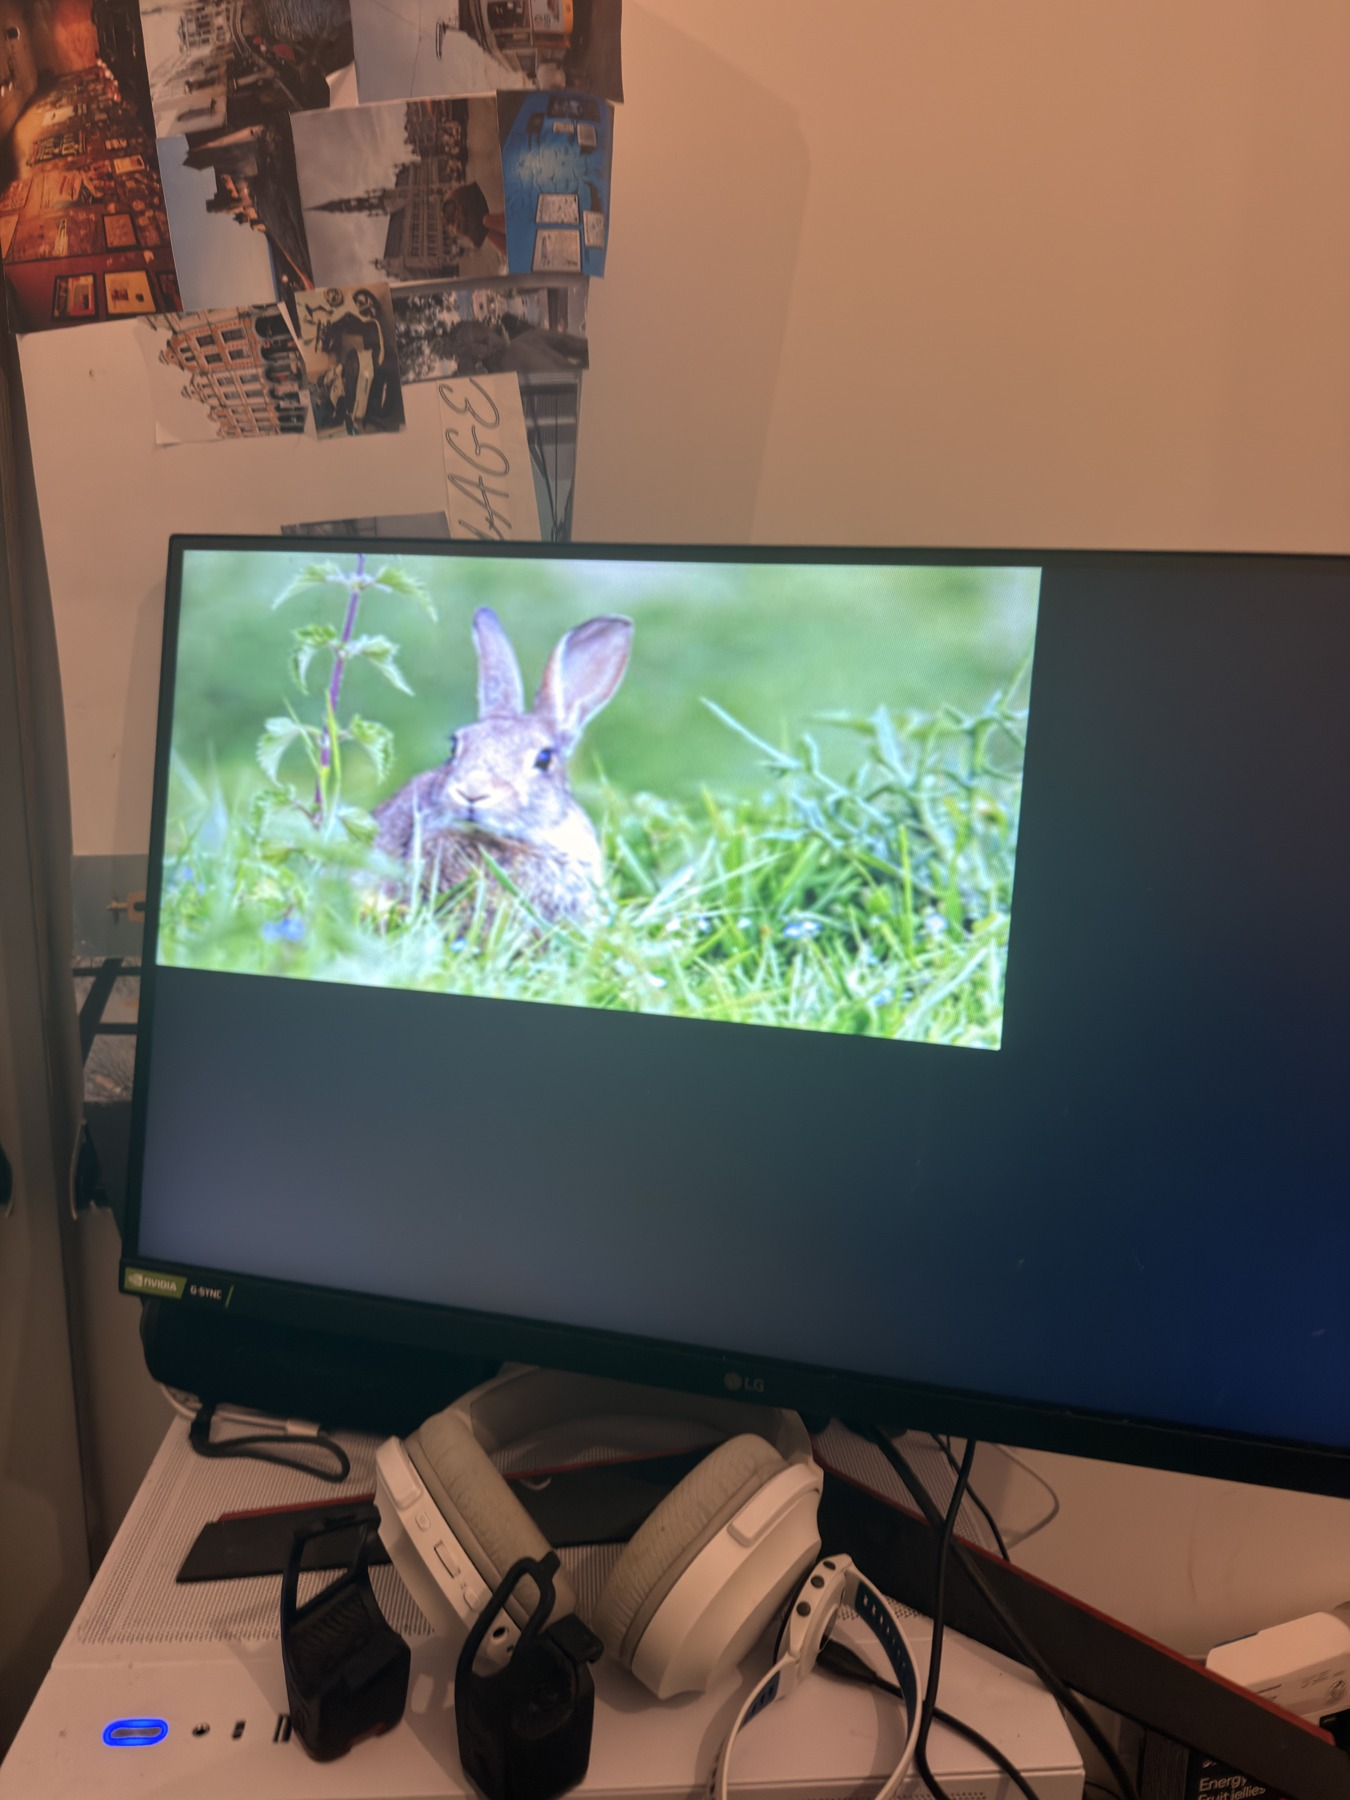
\includegraphics[width=\linewidth,height=7cm,keepaspectratio]{images/affichage_on.jpg}\\
\small SW0 ON : image affichée.
\end{minipage}\hfill
\begin{minipage}{0.47\linewidth}
\centering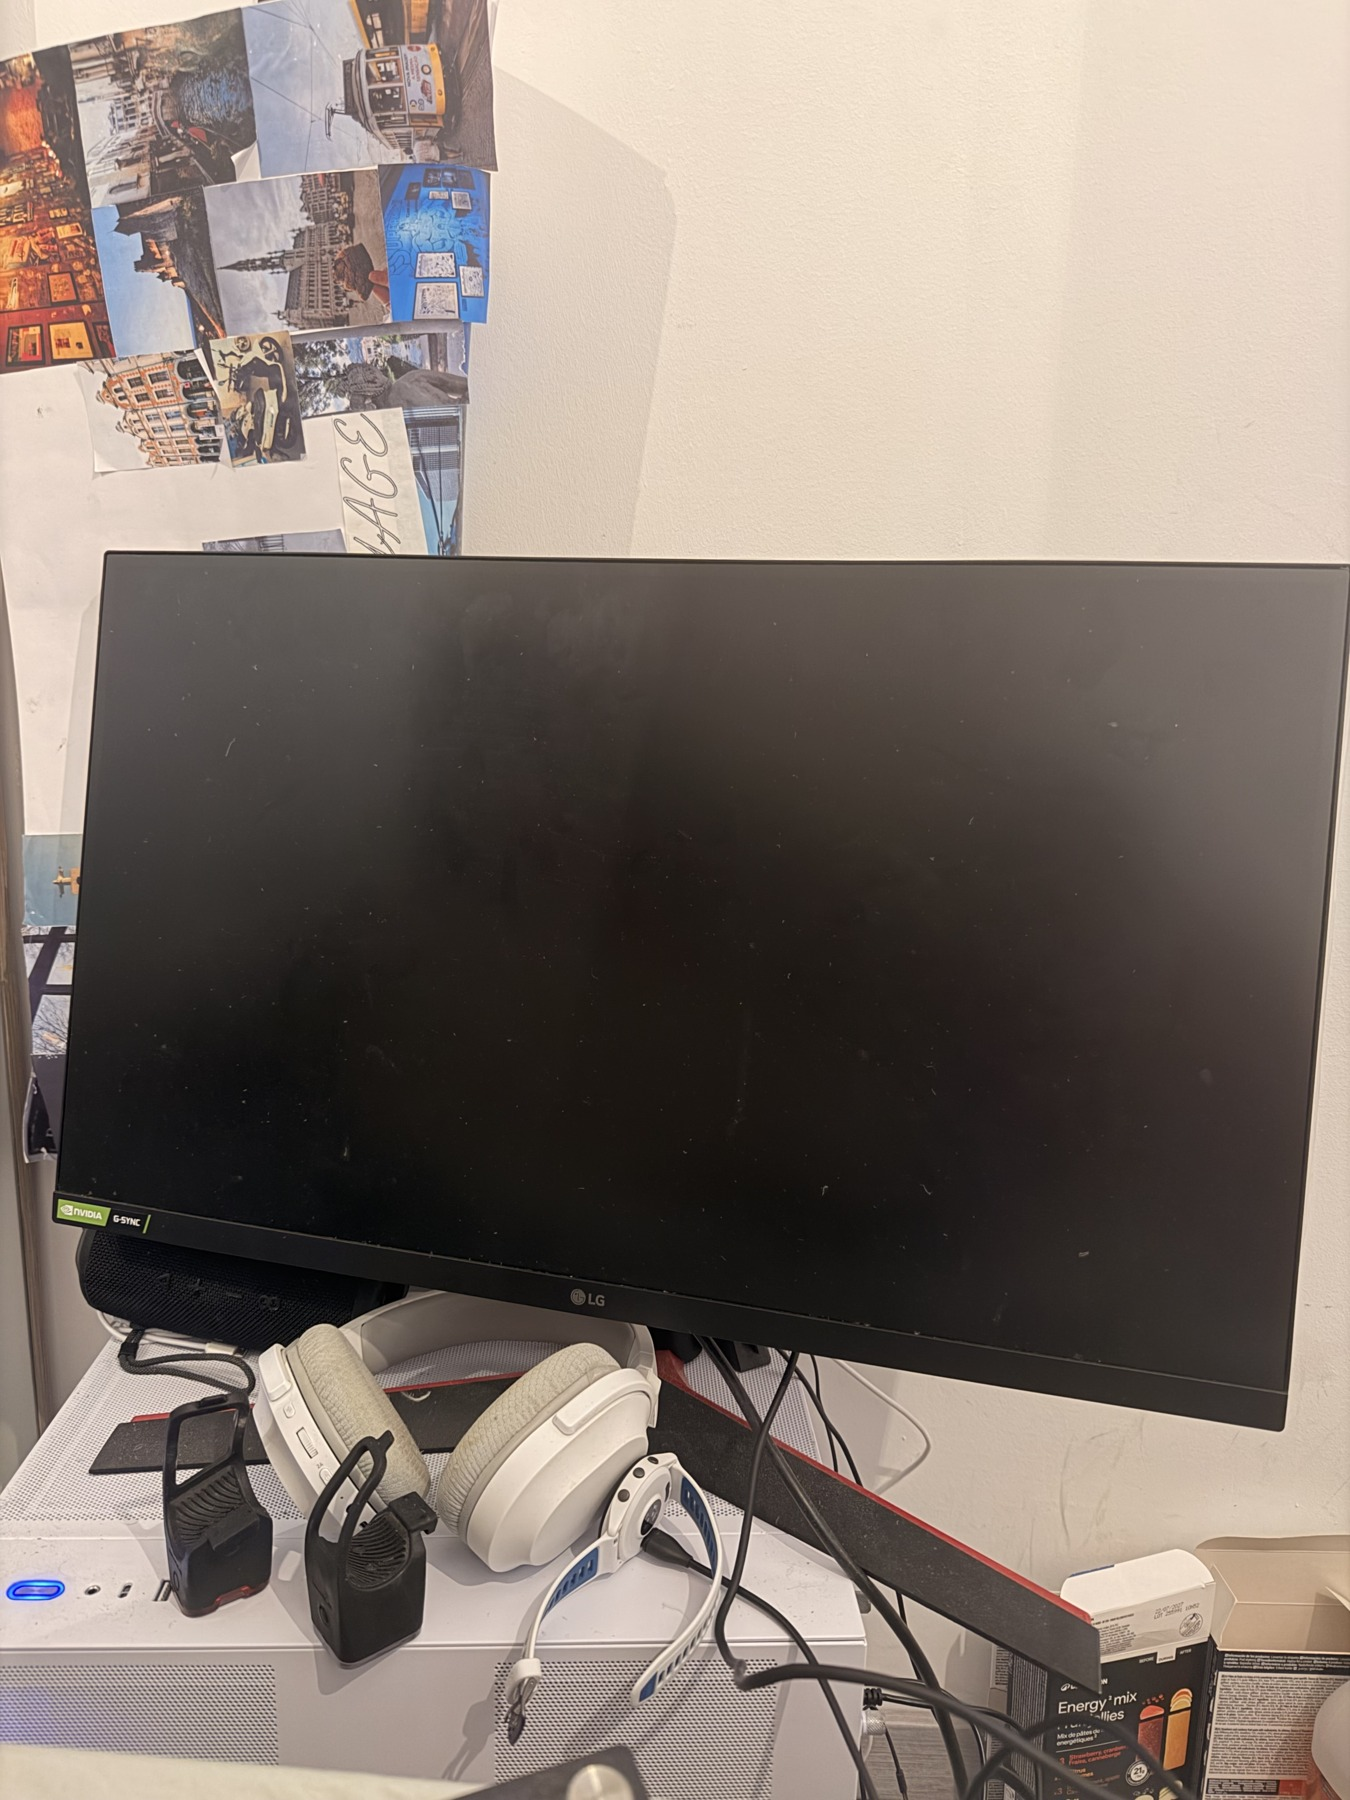
\includegraphics[width=\linewidth,height=7cm,keepaspectratio]{images/affichage_off.jpg}\\
\small SW0 OFF : écran noir.
\end{minipage}
\end{center}

\subsection{Montage et relevés de puissance}
Le montage déclaré est : \textbf{port USB du PC $\rightarrow$ testeur RUI DENG UM25C $\rightarrow$ entrée DC 5 V de la DE10-Nano}. Le testeur observe l'entrée d'alimentation de la plateforme, avec les pertes du câble situé en aval. Il n'isole pas le FPGA, le filtre ou le transmetteur HDMI.

\begin{center}
\begin{tabular}{@{}llrrr@{}}
\toprule
Photographie & SW0 & $U$ (V) & $I$ (A) & $UI$ (W)\\
\midrule
IMG\_0568 & ON & 4,997 & 0,6293 & 3,144612\\
IMG\_0566 & OFF & 4,996 & 0,6240 & 3,117504\\
IMG\_0572 & ON & 5,004 & 0,6301 & 3,153020\\
IMG\_0573 & OFF & 5,005 & 0,6238 & 3,122119\\
\bottomrule
\end{tabular}
\end{center}
Les puissances sont recalculées à partir des valeurs de tension et de courant lisibles sur les photos. La précision d'affichage du testeur ne constitue pas une incertitude métrologique ; les décimales des produits sont conservées pour rendre le calcul reproductible.

\subsection{Puissances moyennes et énergie par image}
La moyenne arithmétique des deux instantanés de chaque état donne :
\[
 \overline P_{\mathrm{ON}}=3{,}14881625\ \mathrm{W},\qquad
 \overline P_{\mathrm{OFF}}=3{,}11981150\ \mathrm{W}.
\]
Ce ne sont pas des moyennes temporelles sur une campagne instrumentée.
\[
 \boxed{E_{\mathrm{image,ON}}\simeq
 \frac{3{,}14881625}{59{,}5238}
 =0{,}0529001\ \mathrm{J/image}
 \simeq52{,}9\ \mathrm{mJ/image}}
\]
Cette énergie correspond à une trame vidéo de sortie comprenant une image de lapin ; il ne s'agit pas d'une mesure isolée de l'énergie de convolution.

\newpage
\section{Discussion et conclusion}
\subsection{Interprétation de la différence ON / OFF}
La différence calculée est :
\[
 \Delta P=29{,}00475\ \mathrm{mW},\qquad
 \frac{\Delta P}{r}\simeq0{,}4873\ \mathrm{mJ/image}.
\]
Le second nombre compare le fonctionnement au reset, ramené au débit nominal ON. Il ne définit pas un débit de traitement dans l'état OFF, où aucune image utile n'est produite.

Le reset modifie plusieurs activités à la fois : balayage utile, mémoire, calcul et interface vidéo. La différence ON/OFF ne peut donc pas être attribuée uniquement au filtre. Elle est petite devant la puissance d'entrée totale, mais quatre instantanés ne permettent pas d'en établir la significativité ou une incertitude robuste.

\begin{center}
\begin{minipage}{0.47\linewidth}
\centering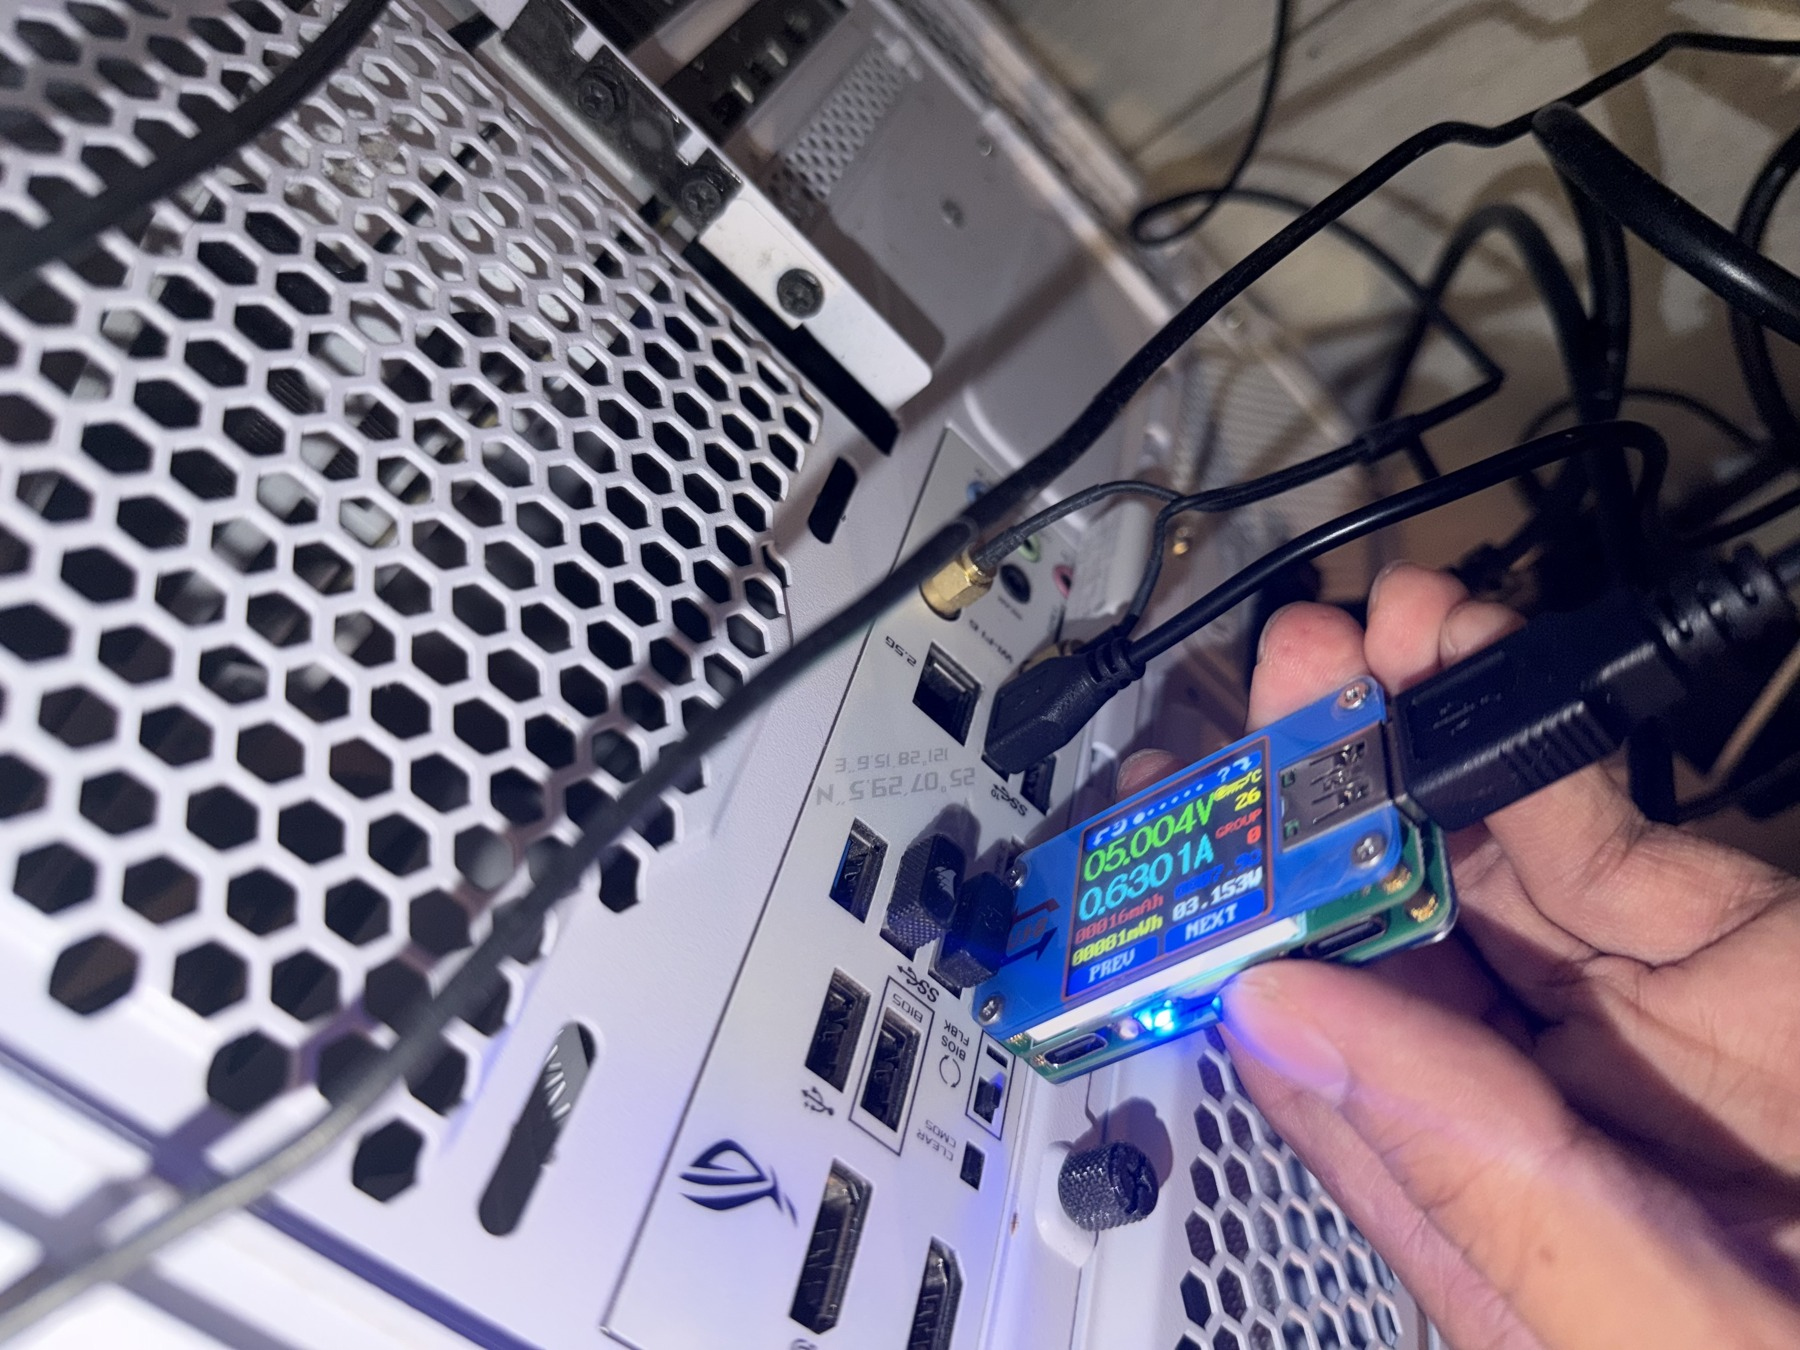
\includegraphics[width=\linewidth,height=5cm,keepaspectratio]{images/mesure_on.jpg}\\
\small IMG\_0572 : ON, 5,004 V et 0,6301 A.
\end{minipage}\hfill
\begin{minipage}{0.47\linewidth}
\centering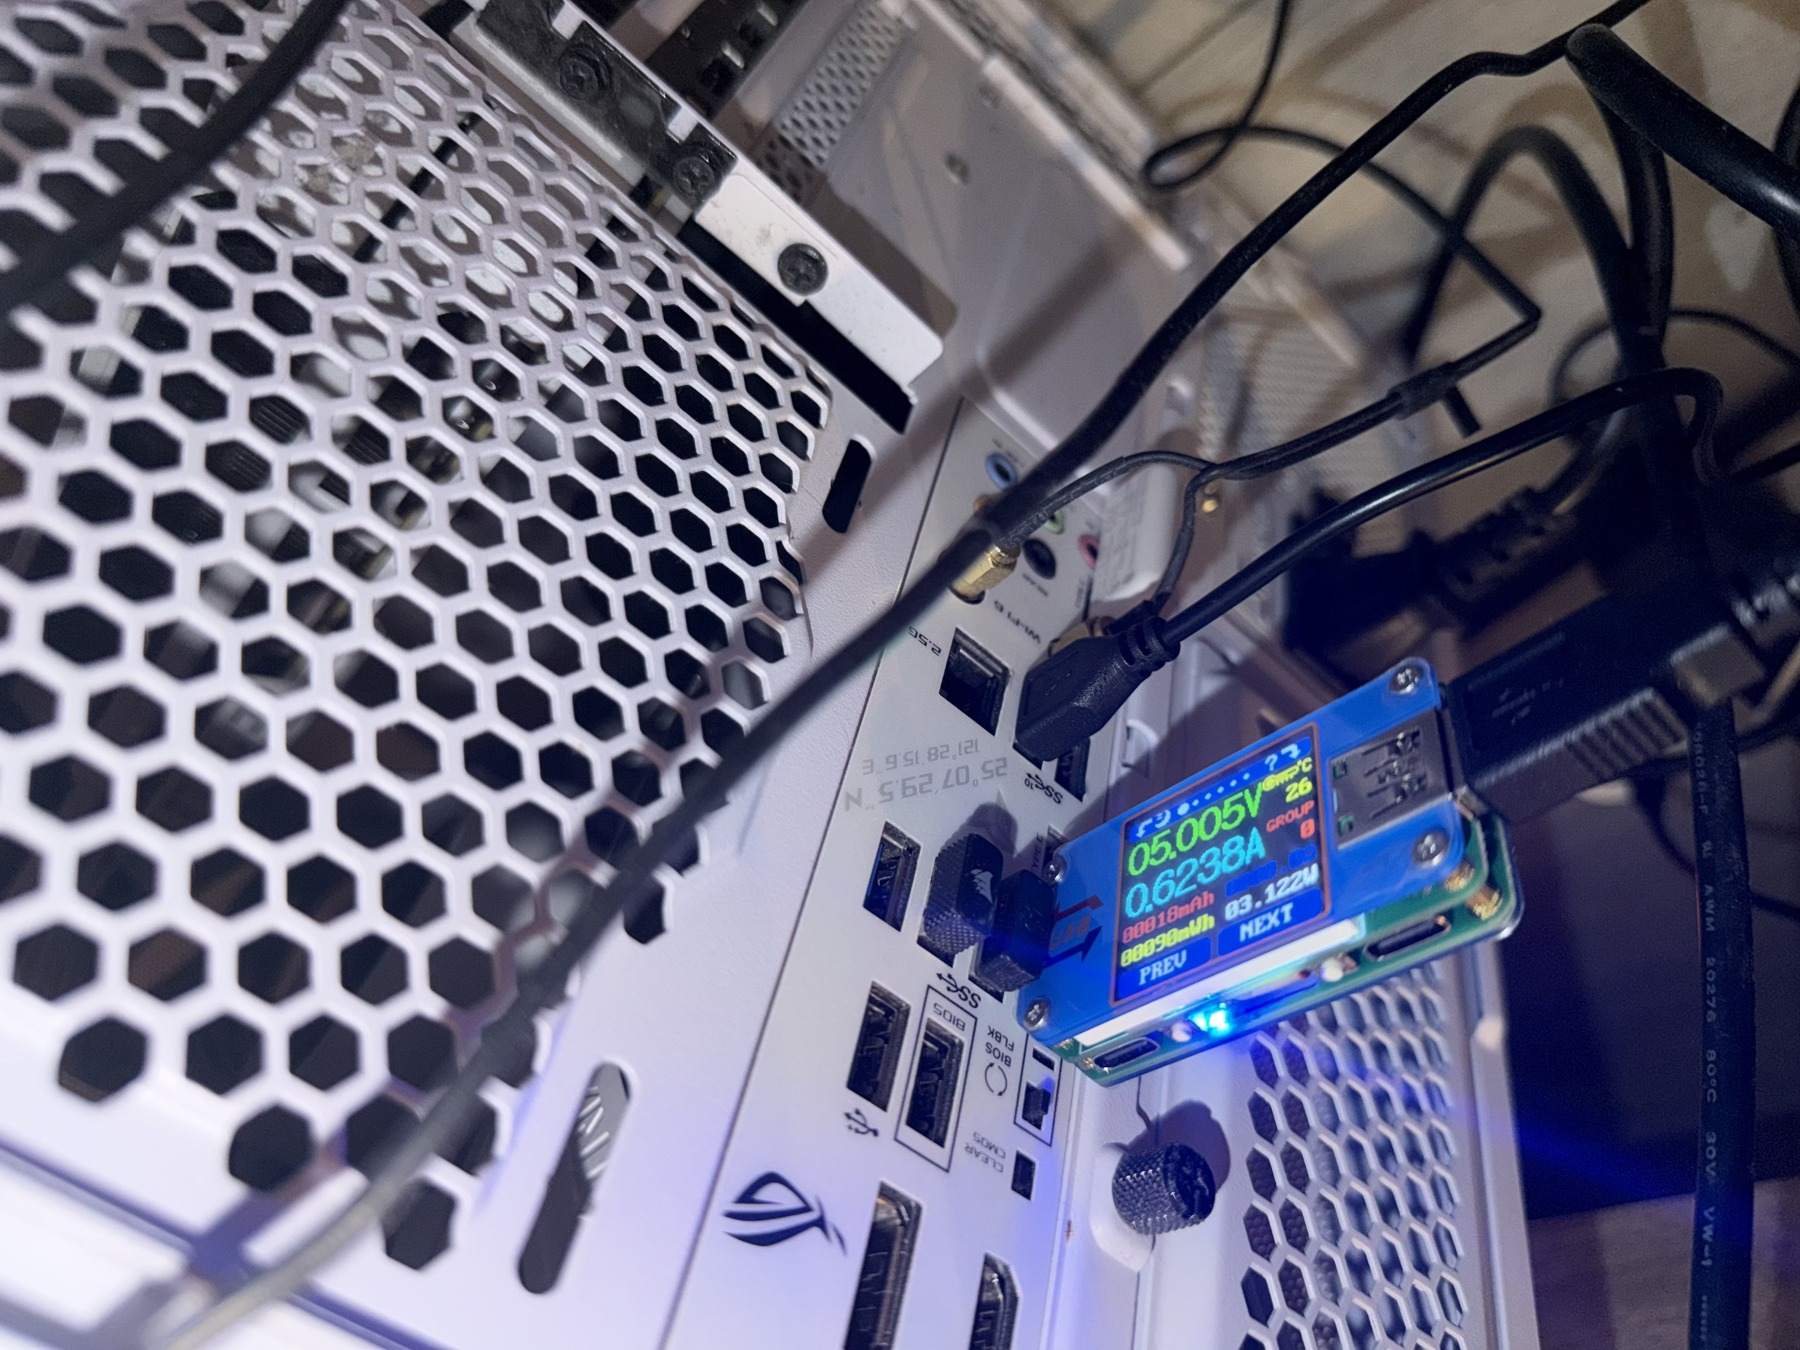
\includegraphics[width=\linewidth,height=5cm,keepaspectratio]{images/mesure_off.jpg}\\
\small IMG\_0573 : OFF, 5,005 V et 0,6238 A.
\end{minipage}
\end{center}

\subsection{Améliorations et travaux restant à réaliser}
Une mesure plus solide intégrerait tension et courant pendant une même durée pour plusieurs répétitions, avec une température stabilisée et des périphériques identiques. Une variante filtre actif / filtre contourné, conservant le même balayage et le même HDMI, isolerait mieux l'effet du traitement que la comparaison avec le reset.

Pour terminer la comparaison architecturale de l'énoncé, il faut compléter les variantes d'addition, de pipeline et de parallélisme, produire des activités représentatives, puis mesurer le débit valide et la puissance. L'exercice 2 demande encore le délai critique et une estimation de puissance propre à l'IP. L'ancien rapport du multiplieur constitue un point de départ, mais son faible niveau de confiance interdit une comparaison énergétique définitive.

\subsection{Conclusion}
La chaîne réalisée stocke une image en ROM, construit un voisinage 3$\times$3, effectue un lissage RGB et génère une sortie HDMI. L'affichage sur carte est documenté. Les relevés conduisent à environ \textbf{3,149 W en fonctionnement} et \textbf{52,9 mJ par trame} au périmètre de l'alimentation, pour un débit nominal de 59,52 images/s.

Ce résultat valide une première caractérisation de la plateforme. Il ne remplace pas les comparaisons d'opérateurs ni la mesure du filtre isolé demandées par les exercices précédents.

\newpage
\section*{Sources et traçabilité}
\begin{enumerate}
\item C. Belleudy, \emph{TP1 : Étude de la consommation d'un core}, énoncé SMUEL302, fichier \path{TP1_M2_2026.pdf}, une page.
\item C. Belleudy, complément au TP1, fichier \path{TP1_M2_2026-2.pdf}, notamment diapositives 5--11, 14--20, 34--43.
\item C. Belleudy, \emph{Estimation et Optimisation de la consommation dans les architectures multicores}, support Moodle \texttt{M2\_LP\_P1\_2025.pdf}, diapositives 8--9, 18 et 20.
\item Projet TP1\_ARCHI, dossier \texttt{github\_DE10\_Nano} : sources classées dans \texttt{exo1}, \texttt{exo2} et \texttt{exo3}, fichier \path{exo3/bitstream/build-info.txt}, photos et \path{exo3/resultat/mesures.csv}.
\item Projet local \path{M2_TP1_Archi/TP1/output_files} : rapports \texttt{TP1.pow.rpt}, \texttt{TP1.pow.summary} et \texttt{TP1.fit.summary}, datés du 29 septembre 2026.
\end{enumerate}

\subsection*{Calcul reproductible à partir des relevés}
\begin{lstlisting}[language=Python]
p_on = (4.997 * 0.6293 + 5.004 * 0.6301) / 2
p_off = (4.996 * 0.6240 + 5.005 * 0.6238) / 2
fps = 25_000_000 / (800 * 525)
e_frame = p_on / fps
delta_p = p_on - p_off
delta_e_frame = delta_p / fps
\end{lstlisting}

\subsection*{Distinction des preuves}
\begin{center}
\begin{tabularx}{\linewidth}{@{}l X@{}}
\toprule
Nature & Ce qu'elle permet d'affirmer\\
\midrule
Sources RTL & Architecture décrite, dimensions, noyau et calendrier nominal.\\
Rapports Quartus archivés & Résultats de la compilation documentée, avec ses contraintes et limites.\\
Photos de l'écran & Présence du lapin en ON et écran noir en OFF.\\
Photos du testeur & Valeurs instantanées de tension et de courant.\\
Calculs de ce rapport & Puissances par produit $UI$, moyennes des relevés et normalisation par le débit nominal.\\
\bottomrule
\end{tabularx}
\end{center}

Le projet de rapport conserve les images utilisées et les relevés bruts. Les autres sources de cours et les projets Quartus restent dans leurs dossiers d'origine.
\end{document}